
\section{Part II - Monovariable control} \label{sec:part2}
In this part of the assignment two new controllers were made to control the pitch and travel rate. A controller for elevation was pre-made and implemented into the Simulink model.
\subsection{Problem 1}
In this problem a PD regulator was added to the system to control the pitch angle \eqref{6a}.
    \begin{equation}\label{PDreg}
       {\tilde{V_d}} = K_{pp}(\tilde{p_c} - \tilde{p}) - K_{pd}\dot{\tilde{p}}
    \end{equation}
    \begin{equation*}
        \ddot{\tilde{p}} = K_1\tilde{V_d}
    \end{equation*}
    \begin{equation}\label{pdotdot}
        \ddot{\tilde{p}} = K_1 K_{pp}(\tilde{p_c} - \tilde{p}) - K_1 K_{pd}\dot{\tilde{p}}
    \end{equation}
To find the transfer function for this system the Laplace transformation with the zero initial condition was used in \eqref{pdotdot}
    \begin{equation*}
        s^2\tilde{p} = K_1 K_{pp}(\tilde{p_c} - \tilde{p}) - s K_1 K_{pd}\tilde{p}
    \end{equation*}
    \begin{equation*}
        \tilde{p}(s^2 + s K_1 K_{pd} + K_1 K_{pp}) = K_1 K_{pp} \tilde{p_c}
    \end{equation*}
    \begin{equation}\label{transf21}
        h_{\tilde{p}}(s) = \frac{\tilde{p}}{\tilde{p_c}}(s) = \frac{K_1 K_{pp}}{s^2 + s K_1 K_{pd} + K_1 K_{pp}}
    \end{equation}
Since \eqref{transf21} is a second order transfer function it could be regarded as a general transfer function for a second order linear system, \eqref{solin}.
    \begin{equation}\label{solin}
        h(s) = \frac{K}{s^2 + 2\zeta\omega_0 + \omega_0^2}
    \end{equation}
These two systems were compared and the corresponding $\omega_0$ and $\zeta$ was found to be
    \begin{equation*}
        \omega_0 = \sqrt{K_1 K_{pp}}
    \end{equation*}
    \begin{equation*}
        2 \zeta \omega_0 = K_1 K_{pd}
    \end{equation*}
    \begin{equation} \label{eq_zeta}
        \zeta = \frac{1}{2} \frac{K_1 K_{pd}}{\sqrt{\omega_0}} = \frac{1}{2} \frac{K_1 K_{pd}}{\sqrt{K_1 K_{pp}}} = \frac{1}{2} \frac{K_{pd}}{K_{pp}}\sqrt{K_1 K_{pp}}
    \end{equation}
A rapidly controlled pitch without oscillating effect was asked for, and therefore a critically damped system was chosen. One condition for second order critically damped systems is $\zeta = 1$. And from \eqref{eq_zeta} the equation was
    \begin{equation*}
       \zeta = 1 = \frac{1}{2} \frac{K_{pd}}{K_{pp}}\sqrt{K_1 K_{pp}}
    \end{equation*}
    \begin{equation}\label{Kpp}
        K_{pp} = \frac{1}{4} K_1 (K_{pd})^2
    \end{equation}
Poles in this transfer function correlate directly to the eigenvalues, which means that choosing values for $K_{pd}$ and $K_{pp}$ will affect the systems behaviour directly. With these equations $K_{pd}$ could be chosen to any value and with the calculated $K_{pp}$ it would still be a critically damped system. After testing out different values, the value which gave the best response to the system was found to be $K_{pd} = 9$, and with \eqref{Kpp} the resulting was $K_{pp} = 11.47$.

\begin{figure}[H]
\graphicspath{Part2_pictures/}
\begin{subfigure}{0.5\textwidth}
    \includegraphics[width=0.9\linewidth]{Part2_pictures/p2p1/Kpd9pitch.eps}
    \caption{$K_{pd}= 9$}
\end{subfigure}
\begin{subfigure}{0.5\textwidth}
    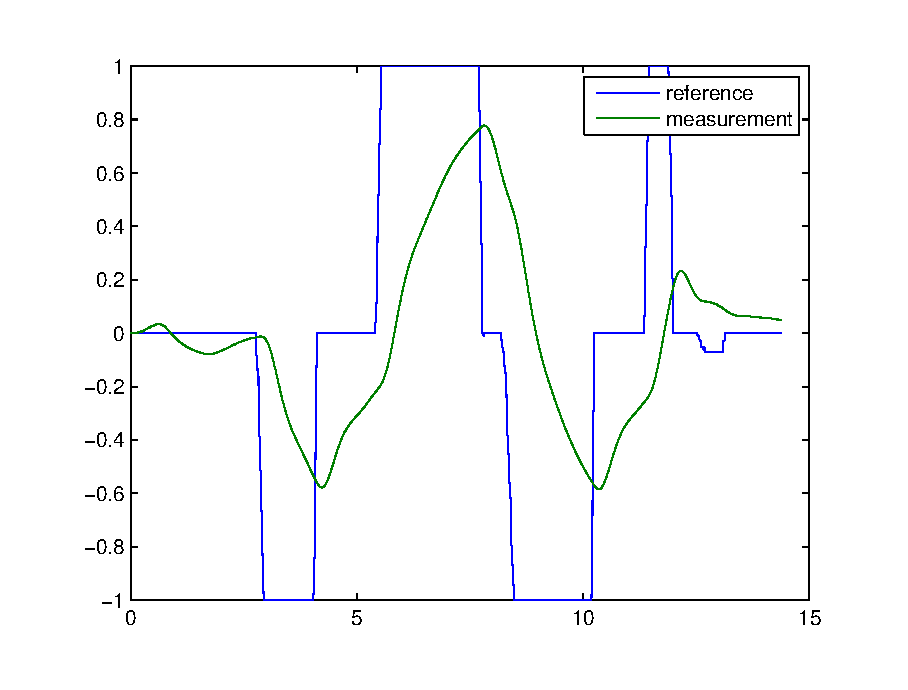
\includegraphics[width=0.9\linewidth]{Part2_pictures/p2p1/Kpd5pitch.eps}
    \caption{$K_{pd}= 5$}
\end{subfigure}
\begin{subfigure}{0.5\textwidth}
    \includegraphics[width=0.9\linewidth]{Part2_pictures/p2p1/Kpd15pitch.eps}
    \caption{$K_{pd}= 15$}
\end{subfigure}
\begin{subfigure}{0.5\textwidth}
    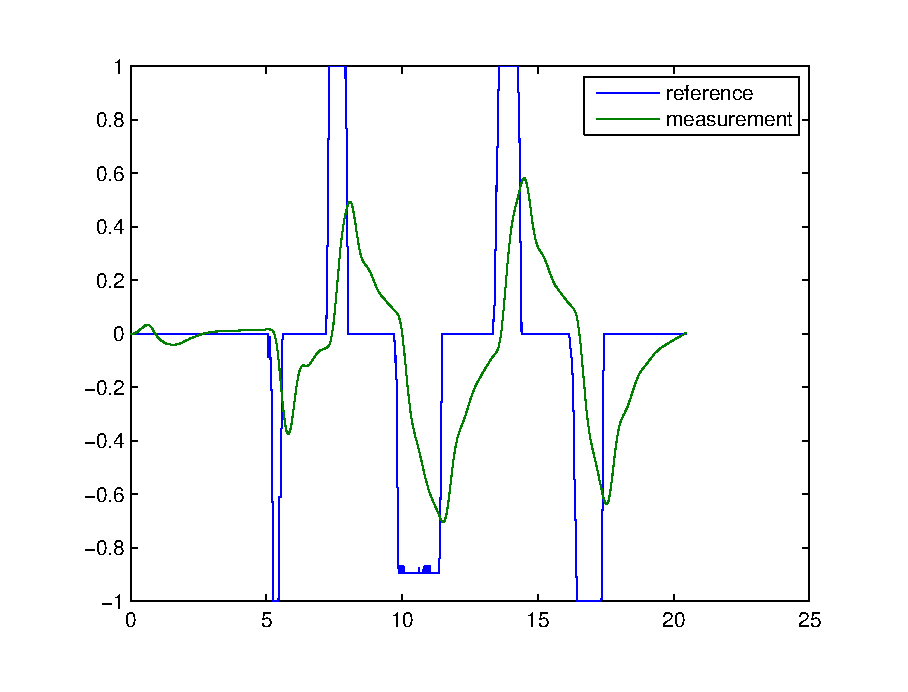
\includegraphics[width=0.9\linewidth]{Part2_pictures/p2p1/Kpd7pitch.eps}
    \caption{$K_{pd}= 7$}
\end{subfigure}
\caption{Different values of $K_{pd}$ for pitch angle}
\end{figure}

\subsection{Problem 2}
In this problem a simple P regulator was added to to the system to control the travel rate.
\begin{equation}\label{eq:lamda_P}
    {\tilde{\rho_c}} = K_{rp} (\dot{\tilde{\lambda_c}} -\dot{\tilde{\lambda}})
\end{equation}
With this equation, \eqref{6c} and the assumption of perfect controlled pitch angle $\tilde{\rho} = \tilde{\rho_c}$ the following equation was found 
\begin{equation*}
    \tilde{\rho_c} = \tilde{\rho} = \frac{\ddot{\tilde{\lambda}}}{K_3}
\end{equation*}
\begin{equation*}
    K_{rp}( \dot{\tilde{\lambda_c}} -\dot{\tilde{\lambda}}) = \frac{\ddot{\tilde{\lambda}}}{K_3}
\end{equation*}
\begin{equation}\label{lamdadotdot}
    \ddot{\tilde{\lambda}} = K_{rp} K_3 (\dot{\tilde{\lambda_c}} -\dot{\tilde{\lambda}})
\end{equation}
To find the transfer function the Laplace transformation with the zero initial condition was used on \eqref{lamdadotdot}
\begin{equation*}
    s\dot{\tilde{\lambda}} = K_{rp} K_3 (\dot{\tilde{\lambda_c}} -\dot{\tilde{\lambda}})
\end{equation*}
\begin{equation*}
    \dot{\tilde{\lambda}}(s + K_{rp} K_3) = K_{rp} K_3 \dot{\tilde{\lambda_c}}
\end{equation*}
\begin{equation}\label{translambdadot}
    h_{\dot{\tilde{\lambda}}}(s) = \frac{\dot{\tilde{\lambda}}}{\dot{\tilde{\lambda_c}}}(s) = \frac{K_{rp} K_3}{s + K_{rp} K_3} = \frac{\rho}{s + \rho}
\end{equation}
Since both $K_{rp}$ and $K_3$ are constants, $K_{rp} K_3$ is simply rewritten as $\rho$ and the resulting transfer function is on the characteristic form of a low pass filter. To get a stable system $\rho$ must be in the left half plane, and therefore $K_{rp}<0$. $K_{rp}$ was tested for values that made the helicopters response fast and accurate, and the best response was found at $K_{rp} = -1$. The helicopter would still rotate with a small constant velocity, but this was expected as to get rid off stationary deviation an integral effect is needed. 

\begin{figure}[H]
\graphicspath{Part2_pictures/}
\begin{subfigure}{0.5\textwidth}
    \includegraphics[width=0.9\linewidth]{Part2_pictures/p2p2/Krp05travelrate.eps}
    \caption{$K_{rp}= -0.5$}
\end{subfigure}
\begin{subfigure}{0.5\textwidth}
    \includegraphics[width=0.9\linewidth]{Part2_pictures/p2p2/Krp09travelrate.eps}
    \caption{$K_{rp}= -0.9$}
\end{subfigure}
\begin{subfigure}{0.5\textwidth}
    \includegraphics[width=0.9\linewidth]{Part2_pictures/p2p2/Krp1travelrate.eps}
    \caption{$K_{rp}= -1$}
\end{subfigure}
\begin{subfigure}{0.5\textwidth}
    \includegraphics[width=0.9\linewidth]{Part2_pictures/p2p2/Krp3travelrate.eps}
    \caption{$K_{rp}= -3$}
\end{subfigure}
\caption{travel rate shown with different values for $K_{rp}$}
\end{figure}

